\documentclass[12pt,letterpaper]{article}
\usepackage{fullpage}
\usepackage[top=2cm, bottom=4.5cm, left=2.5cm, right=2.5cm]{geometry}
\usepackage{amsmath,amsthm,amsfonts,amssymb,amscd}
\usepackage{lastpage}
\usepackage{enumerate}
\usepackage{fancyhdr}
\usepackage{mathrsfs}
\usepackage{xcolor}
\usepackage{graphicx}
\usepackage{listings}
\usepackage{hyperref}
\usepackage{pdfpages}


\hypersetup{%
  colorlinks=true,
  linkcolor=blue,
  linkbordercolor={0 0 1}
}
 
\renewcommand\lstlistingname{Algorithm}
\renewcommand\lstlistlistingname{Algorithms}
\def\lstlistingautorefname{Alg.}

\lstdefinestyle{Python}{
    language        = Python,
    frame           = lines, 
    basicstyle      = \footnotesize,
    keywordstyle    = \color{blue},
    stringstyle     = \color{green},
    commentstyle    = \color{red}\ttfamily
}

\setlength{\parindent}{0.0in}
\setlength{\parskip}{0.05in}
\begin{document}






Foundations of Applied Math\\
 HW \#8 Resume, Website draft + Monte Carlo Problem\\
 Due Friday, Nov. 6 by 7 am
 
\textbf{Reminder} You need to turn in a .zipped folder that contains your .tex file, your image files, your python files, your Excel file(s), and the tex file must compile.
Rename the .tex file: HW8$\_$YourLastName.tex and call the folder which you will compress: HW8$\_$YourLastName


\begin{enumerate}

\item Create a new resume or update yours. Enclose a pdf of your resume in your HW folder. You can write your resume in Word and then save it as a pdf. I would expect that you'd do it in Word.
See this page for guidance: \url{https://coopsandcareers.wit.edu/resources/resume-guide/}  
\\
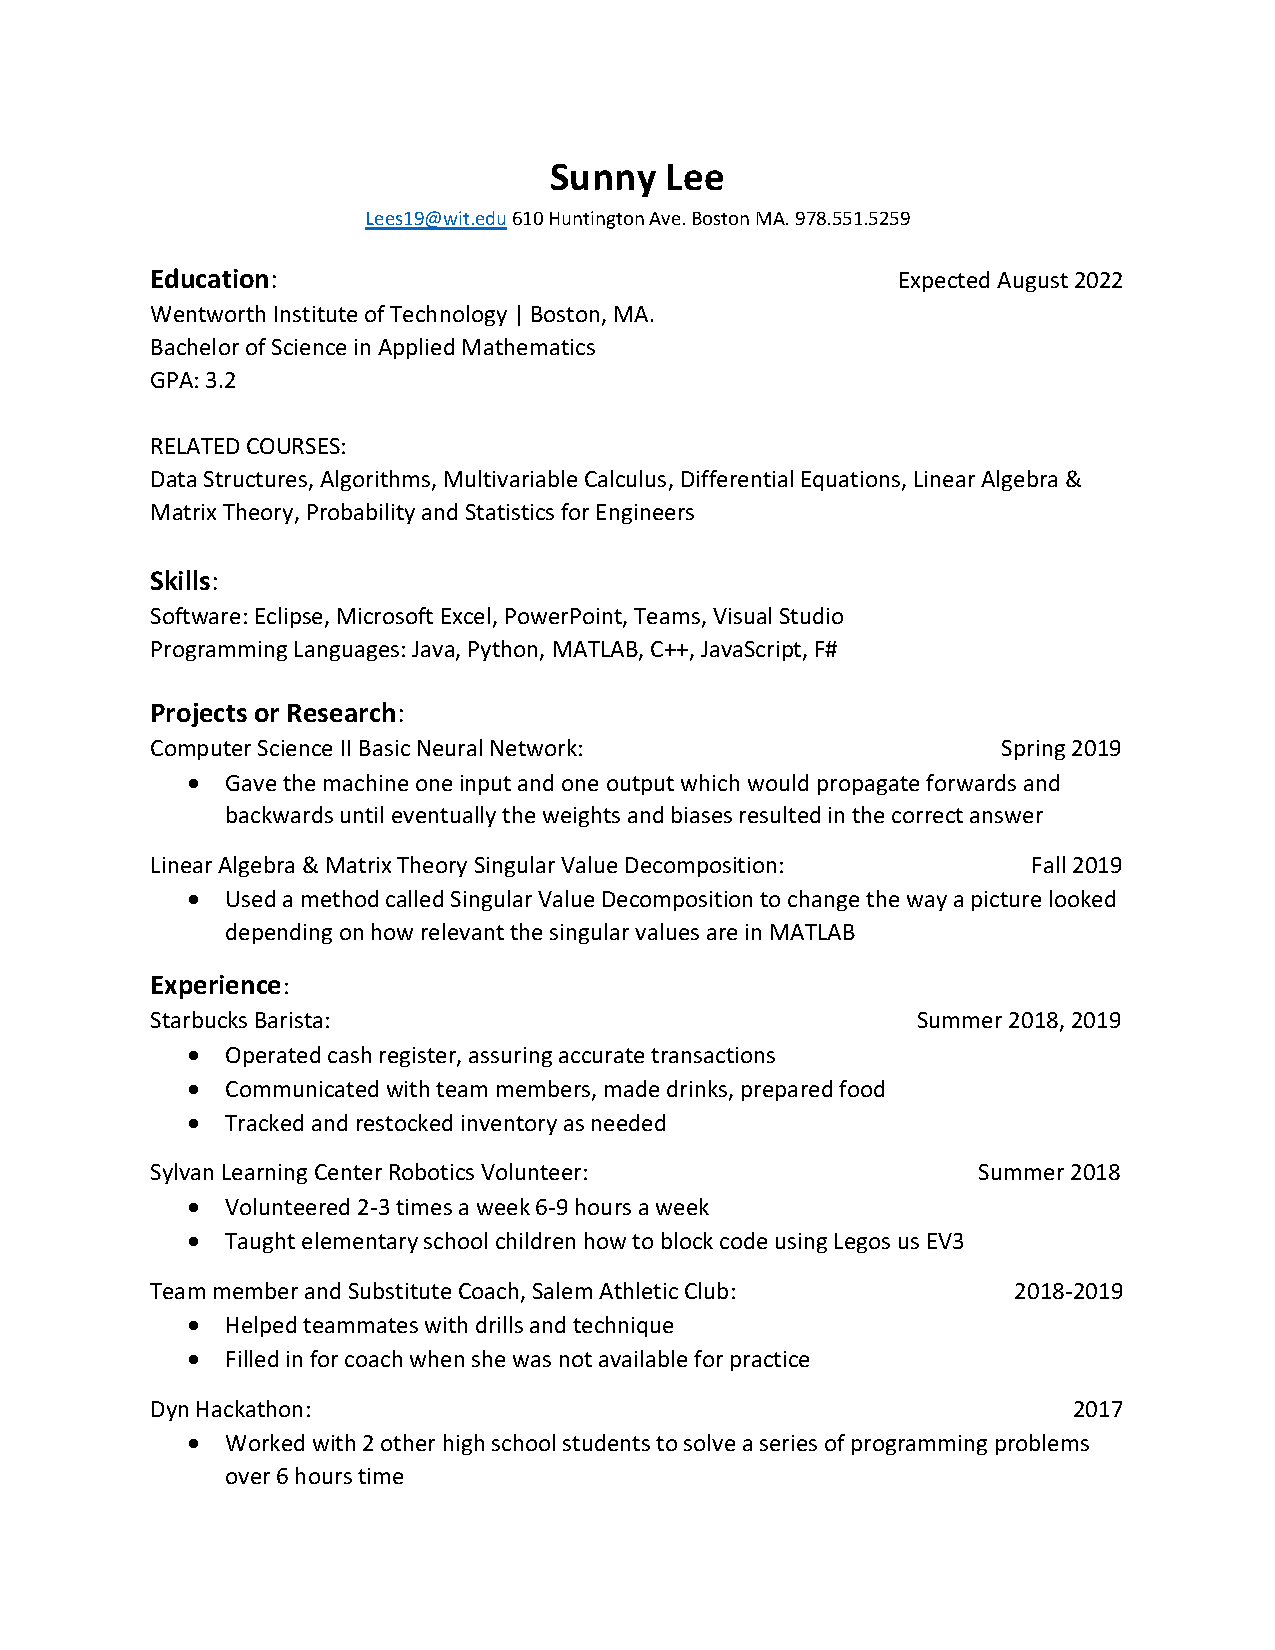
\includepdf[pages=-]{Lee_Resume.pdf}

\item Per the syllabus you need to do a website. For HW 8 your website is a draft website.

\textbf{Please note that your website that you are submitting right now is a draft and is just part of this HW.}

\textbf{Per the syllabus, I will ask you to turn in a final version by Study Day which is the day after the last day of classes.}

 The purpose of this assignment is to give you an early start with your graduation requirement.  You will have to turn in an updated version of this or a new website you may make before you graduate.  You show this in the course Applied Math Final Year Research.  
Your website needs to include your resume (question 1) 

What you need to turn in here is the url of your website.  Just paste the URL into the text box when you submit HW8 or here:





Most students do this using Wix. Here is how to get started: \url{https://www.wix.com/}
\begin{itemize}

\item You will need to demonstrate purposeful inclusion of meaningful, professional content.

\item A Navigation bar allowing the user to get back to the main pages from anywhere on the site.

\item Have a uniform style of pages

\item All images that are relevant to the understanding of the document have alternative text.

For the alt text see: \url{https://support.wix.com/en/article/about-hover-boxes}

(alt text is text you supply for an image so that a screen reader for someone who is visually impaired can read it aloud.)
\item Title of webpage for the title bar

\item  Appropriate contact information (LinkedIn, email, etc.)  Be careful not to include home address/phone number or other information.

\item Highlights of your resume written directly into webpage 

For instance, you may chose to highlight relevant work experience in co-ops, awards, special skills

\item  Link to PDF of your resume

\item  Include at least one image. 

One image should be a `branding image,' which could be an image of you or one symbolic of your work.
Again be careful of the image you chose to make sure it is professional and is in line with the amount of
internet presence you want to provide.

\item Showcase of completed projects 
You may not have this yet but just have a place holder for this.

\end{itemize}
Here are examples of a few prior  students (who updated their webpages when they were in their last years).

\url{https://erichenschel7.wixsite.com/mathatthehelm}

\url{ https://whyweiway.wixsite.com/website}

\url{ https://ellenbuttseb.wixsite.com/website}
\vskip1em
Website:
\url{https://lees191.wixsite.com/website}

\item Consider $$\frac{x^2}{4} + \frac{y^2}{16} + \frac{z^2}{9}=1$$.
\begin{enumerate}[a)]
\item Use Geogebra  (see \url{https://www.geogebra.org/3d?lang=en}  to plot this surface. Include the plot here.\\
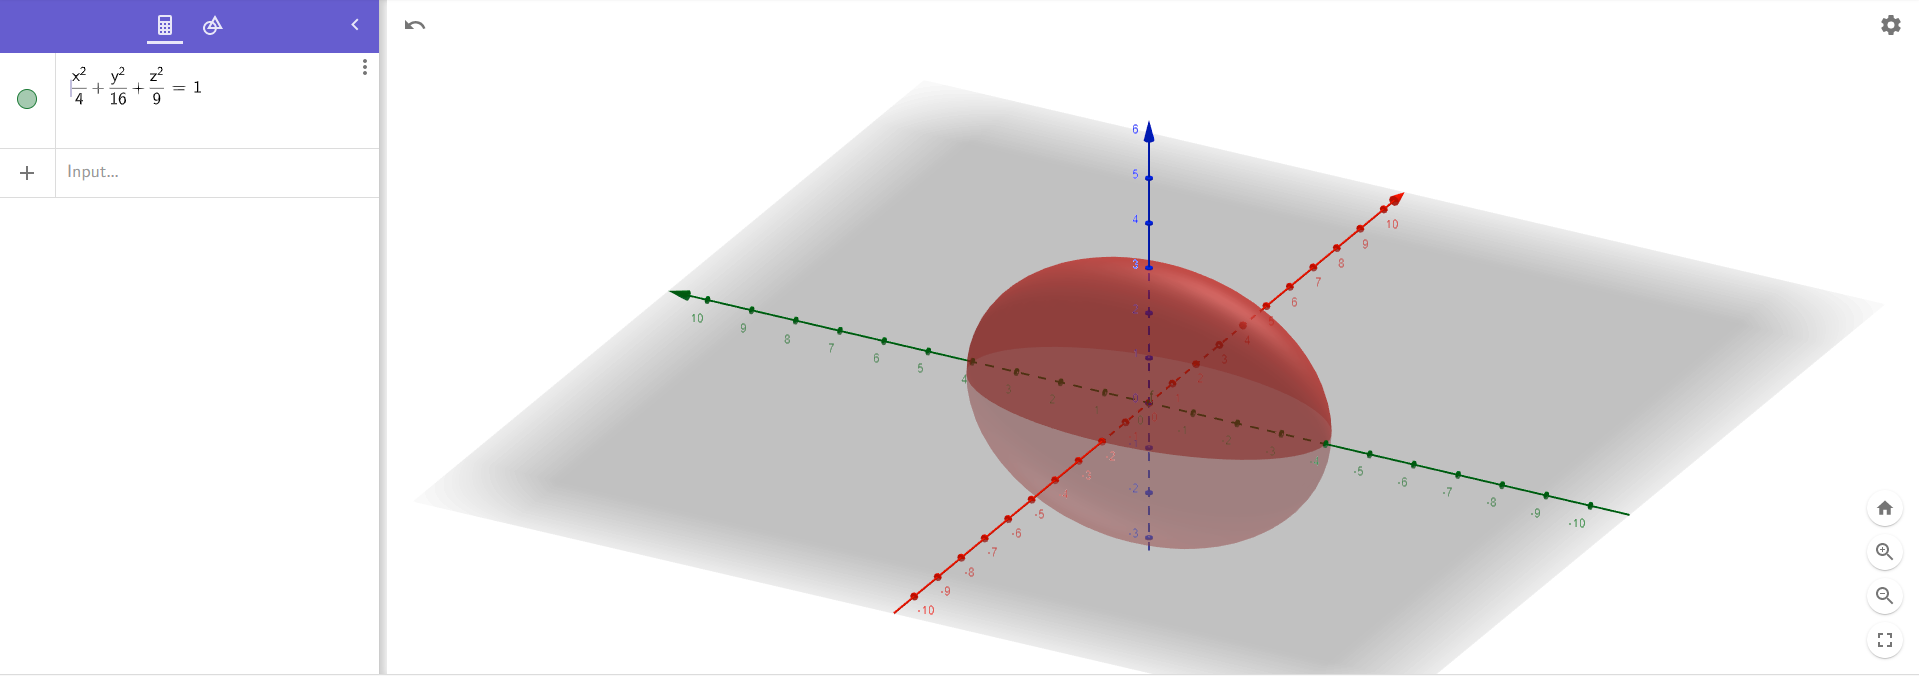
\includegraphics[scale = .3]{ellipsoid.png}\\
\item Using a Monte Carlo simulation, use python to write an algorithm to approximate the volume inside this shape.
\\The python file montecarlo.py is included. \\
To use the monte carlo method, we first solve the function in terms of $z$. Solving for 
$z$, our function is already split into above and below the $z$ axis. We can take 
one of those and create a box around our function. Using the np.where function, 
we can find how many of our randomly generated points land inside the elilpsoid, 
take that over the amount of points we have randomly generated, and multiply double 
that times the volume of the box we made and our estimate is: 

\includegraphics[scale = .8]{montecarlo.png}\\

Which we can check against the formula for an ellipsoid: $V = \frac{4}{3}\pi abc$ 
where $a$, $b$, $c$ are the axis of the ellipsoid. Using the formula for the volume, 
we estimate $V = \frac{4}{3}\pi \cdot 2\cdot4 \cdot3 \approx 100.53$ which is quite 
close to our approximation. 
\end{enumerate}


\end{enumerate}
\end{document}